%!TEX root = ../Thesis.tex
%! Author = JB
%! Date = 22.05.2020


\section{Entity-Relationship Diagramm \textcolor{blue}{[Jonathan Brockhausen]}}

In \cref{fig:erd} ist das zugrundeliegende Entity-Relationship Diagramm dargestellt.

\begin{figure}[h!!]
    \centering
    \begin{minipage}[t]{1\textwidth}
        \caption{ERD des Projekts}
        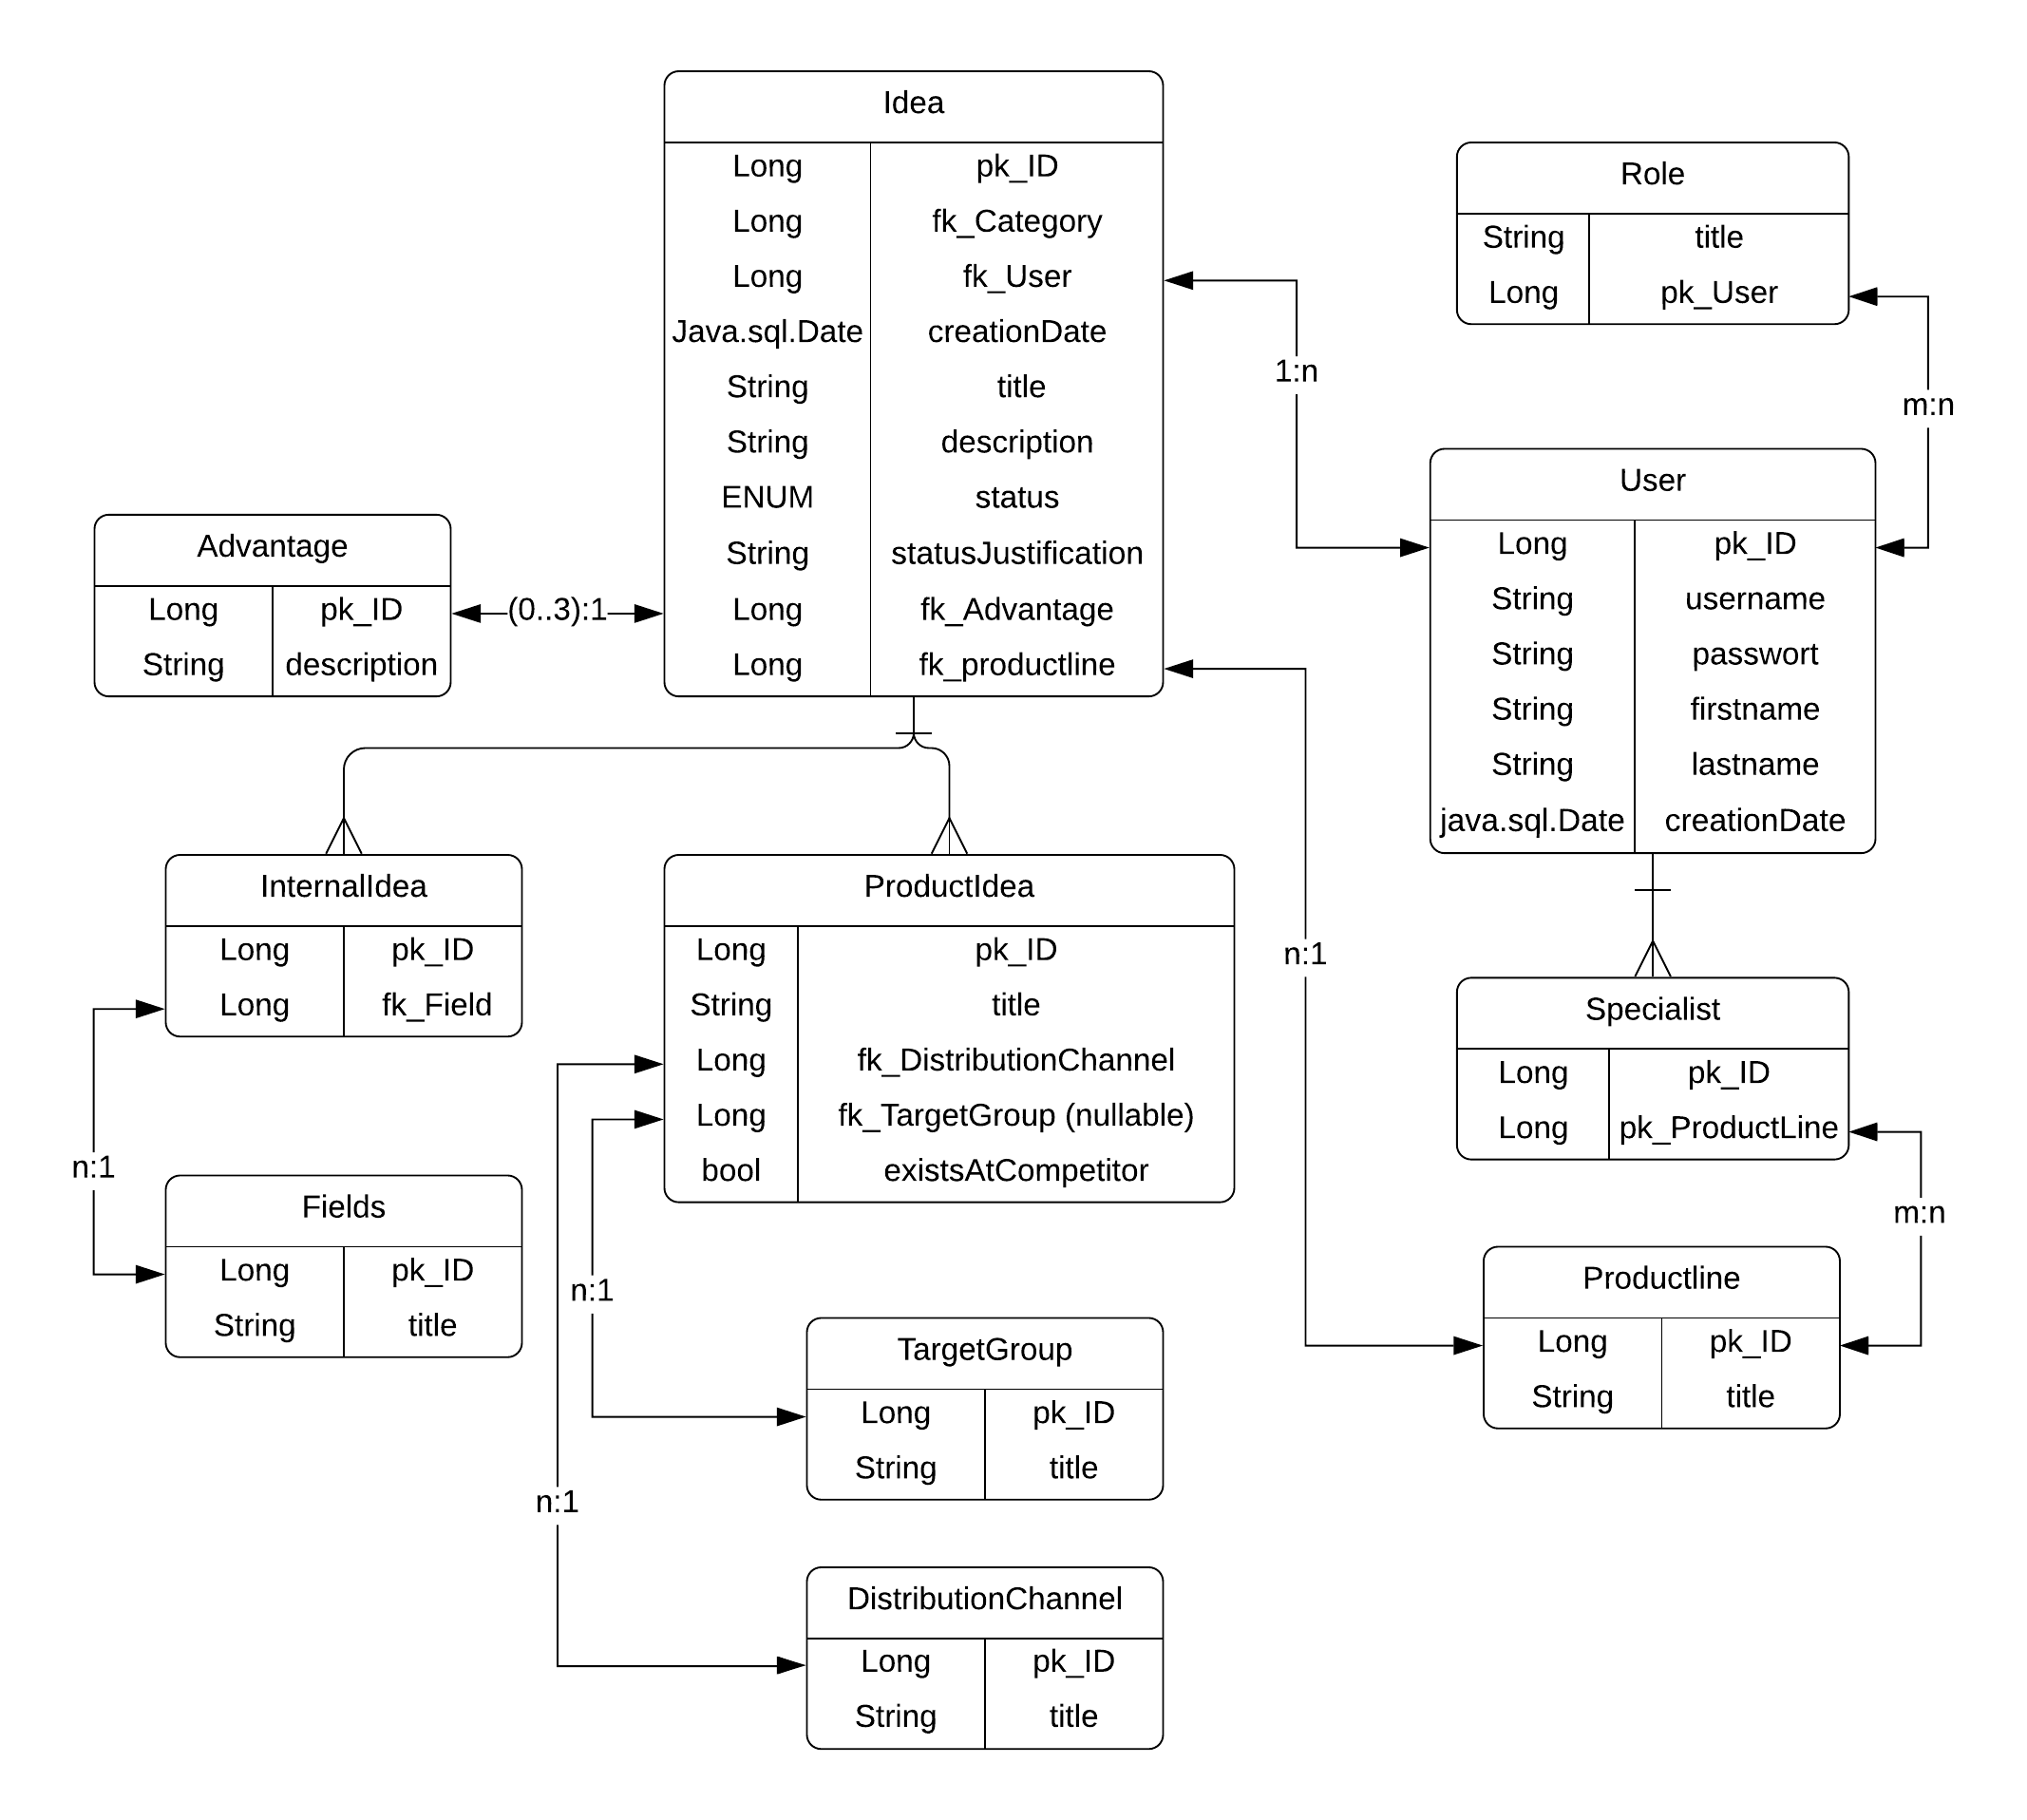
\includegraphics[width=1\textwidth]{img/erd.png}\\
        \source{Eigene Darstellung}
        \label{fig:erd}
    \end{minipage}
\end{figure}

Dieses Diagramm wurde im Programm in der Datenbank umgesetzt. Im Folgenden werden einige Design-Entscheidungen erläutert.\\
\textbf{Zuordnung von Fachspezialisten und Ideen}\\
Um die automatische Zuordnung von Fachspezialisten zu Ideen umzusetzen, haben wir die Produktsparte als Zuordnungskriterium herangezogen.
Die Klasse des Fachspezialisten erbt vom der Klasse des Benutzers mit der zusätzlichen Eigenschaft, dass ihm eine oder mehrere Produktlinien zugewiesen sind.
Einer Produktsparte können mehrere Fachspezialisten zugeordnet sein. Mit dieser m:n-Beziehung erreicht das Programm die größtmögliche Flexibilität.
Jeder Idee (Intern und Produkt) ist eine Produktsparte zugeordnet. Aus den Projektanforderungen ergeben sich mehrere Produktsparten, die bei der Auslieferung bereits vorhanden sind.
Da interne Ideen gemäß der Anforderungen keine Produktsparte besitzen, bekommen Sie die dem Benutzer verborgene Produktsparte \glqq{}INTERNAL\grqq{} zugewiesen. Diese ermöglicht für interne Ideen dieselbe Logik zu verwenden.
Durch diese Umsetzung ist auch eine Erweiterung um weitere Ideenkategorien ohne Änderungen am übrigen Programm möglich.\\
\textbf{Umsetzung von Status}\\
Wir haben uns dagegen entschieden, den Status in eine eigene Entität im Sinne des ERD auszulagern.
Erweiterungen und Änderungen der Status im Echtbetrieb erfordern dann zwar unter Umständen an einigen Stellen Änderungen in der Programmlogik aber die enum bieten insgesamt Performancevorteile gegenüber der Auslagerung als vollwertige Entität und sind leichter im Code umzusetzen.\\
\textbf{Vererbung von Ideen zu interne und Produktidee}\\
Das Anlegen von Klassen mit Vererbung (wie im Projekt bei Ideen und Usern) kann in relationalen Datenbanken zu zwei Schwierigkeiten führen:
\begin{enumerate}
    \item {Lese- und Speicherzugriffe betreffen mehrere Tabellen und erfordern Joins. Das kann zu unübersichtlichen Strukturen und SQL-Kommandos sowie zu geringerer Performance führen}
    \item {Nicht-polymorphe Abfragen (z.B. Namen/Preise nur der Getraenke) sind umständlich (z.B. Unterscheidung per Diskriminator)\footnote{vgl. \cite{Horn2007}}}
\end{enumerate}
Durch die Verwendung von Hibernate mit seiner nativen Java-Integration und die Vermeidung von hardcodeten SQL-Statements im Code, fallen diese Punkte kaum ins Gewicht. Die Struktur der Vererbung ermöglicht es darüber hinaus sogar weitere Kategorien von Ideen anzulegen.


